\documentclass[dvipdfmx]{jsarticle}
\usepackage[dvipdfmx]{graphicx}
\usepackage{amsmath, amssymb}
\usepackage{mathtools}
\usepackage{here}
\renewcommand{\thefigure}{\thesection.\arabic{figure}}
\setcounter{section}{3}
\setcounter{figure}{15}

\begin{document}

\section*{3.4 離散時間モデル}



多くの場合,時変インパルス応答チャネルモデルは複雑すぎて,単純な解析は不可能である.この場合,広帯域マルチパスモデルの離散時間近似を使用することができる.Turinが[3]で開発したこの離散時間モデルは,特にスペクトラム拡散システムやRAKE受信機の研究に有用であり,第13章で取り上げることとする.この離散時間モデルは,図3.16に示すように,孤立した点状散乱体の構成からなる物理的な伝搬環境に基づいている.このモデルでは,マルチパス成分はサブパスクラスタを形成すると仮定し,近似遅延$\tau_n$を持つ任意のサブパス上の受信パスは結合され,遅延$r_n$と$r_m$を持つ異なるサブパスクラスタ上の受信パスは,$|r_n - r_m|> 1 / B$(ここで$B$は信号帯域幅を表す)を分離できるとしている.

\begin{figure}[H]
\begin{center}
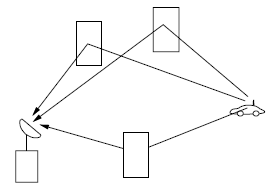
\includegraphics[width=0.65\linewidth]{"./spring_lec/pointScatterChannelModel.png"}
\end{center}
\caption{点状散乱体チャネルモデル}
\end{figure}

(3.6)のチャネルモデルは,これらのサブパスクラスターの固定数$N + 1$を含むように修正される.

\begin{equation}\label{}
c(\tau;t) = \sum^N_{n=0} \alpha_n (t)e^{-\jmath \phi_n (t)} \delta(\tau - \tau_n (t))
\tag{3.64}
\end{equation}

したがって,与えられた$t$に対する受信信号の統計量は,$\{\tau_n\}^N_0, \{\alpha_n\}^N_0, および\{\phi_n\}^N_0$の統計量によって与えられる.
このモデルは,以下のように離散時間近似を用いてさらに単純化することができる.固定された$t$に対して,時間軸は$MT \geq \sigma_{T_m}$($\sigma_{T_m}$は経験的に導出されたチャネルのrms遅延広がり)となるように$M$個の等間隔な持続時間$T$に分割される.図3.17に示すように,サブパスは$M$個の時間間隔ビンのうちの1つに位置するように制限される.この離散的なモデルのマルチパスの広がりは$MT$であり,パス間の分解能は$T$である.この分解能は送信信号の帯域幅に基づく($T \approx 1 / B$).$n$番目のビンの統計量は,$r_n(1 \leq n \leq M)$は,$n$番目のビンにマルチパス成分が存在するかどうかの二値指標である.したがって,$r_n$は$n$番目のビンにマルチパス成分が存在する場合は1,それ以外は0である.$r_n = 1$の場合,このマルチパス成分に対応する振幅と位相である$(a_n, \theta_n)$は,経験的に決定された分布に従う.この分布は,伝搬環境の異なる場所での各$n$の$(a_n, \theta_n)$のサンプル平均によって得られる.$n = m$の$(a_n,\theta_n)$と$(a_m,\theta_m)$の経験分布は一般に異なり,同じ系列のフェージングであっても異なるパラメータ(例えば,異なる係数kを持つライスフェージング)に対応するか,あるいは全く異なるフェージング分布(例えば,$n$番目のビンではレイリーフェージング,$m$番目のビンでは仲上フェージング)に対応する可能性がある.

\begin{figure}[H]
\begin{center}
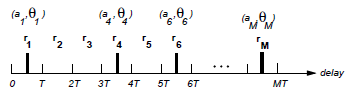
\includegraphics[width=0.75\linewidth]{"./spring_lec/discreteTimeApproximation.png"}
\end{center}
\caption{離散時間近似}
\end{figure}

これで,1つのスナップショットに対する離散時間近似の統計モデルは完成する.一連のプロファイルは,チャネルのインパルス応答が変化するにつれて,時間経過とともに信号をモデル化する.したがってこのモデルは,プロファイルのそれぞれ(等価に,各$t$について)についての$(\tau_n,\alpha_n,\phi_n)$一次統計だけでなく,時間的および空間的相関(マルコフを仮定)を考慮しなければならない.このモデルの詳細と,Nと$(\tau_n, \alpha_n, \phi_n)$に対する経験的に得られた分布は,[3]に記載されている.

\end{document}